\section{Methodology}
\begin{figure*}[ht]
    \centering
    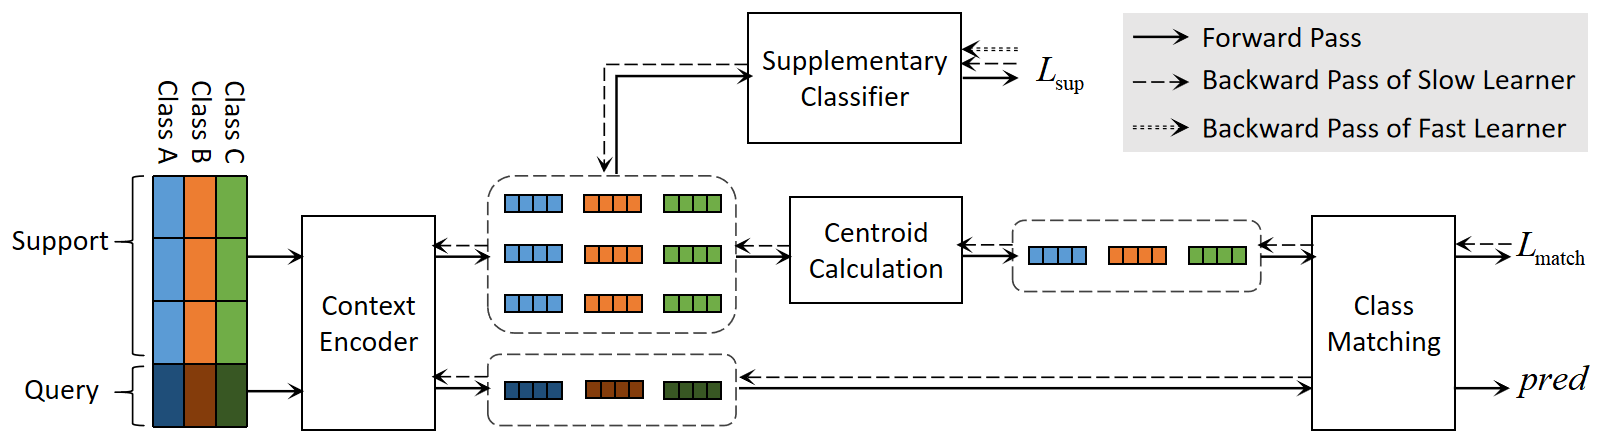
\includegraphics[width=16cm]{model.png}
    \caption{The structure and learning process of the MME framework}
    \label{fig:model}
\end{figure*}
%\KZ{Make figure \ref{fig:model} bigger, fonts bigger too. OK}
In this section, we describe our proposed MME framework in detail.
The MME framework is a novel meta-learning framework which enhances metric-learning based meta methods with a supplementary classifier scheduled by a fast-slow learner strategy. The structure and learning procedure of the MME framework is illustrated in Figure \ref{fig:model}. In \ref{sec:structure} we present the structure of the MME framework. In \ref{sec:process} we show MME's meta-learning process.
\subsection{The structure of MME}
\label{sec:structure}
As is shown in \ref{fig:model}, the structure of MME framework consists of three main parts: context encoder, class matching and supplementary classifier.
\subsubsection{Context encoder}
A support or query instance can be represented as a triple $(s, e, r)$, where $s$ is the sentence containing two entities $e=(e_1,e_2)$, and $r$ is the relation between $e_1$ and $e_2$. $r \in R$ where $R=\{r_1,...,r_N\}$ is the set of all candidate relation classes within one task and $N$ is the number of candidate classes.
Sentence $s=\{c_0,..., c_i, ... c_{T-1}\}$ is of length $T$, where $c_i$ represent the one-hot vector of the $i^{th}$ character.
In context encoder, each $c_i$ is mapped into a $d_c$ dimensional character embedding $\bm{x_i}$.
To integrate positional information of $e_1$ and $e_2$ to each character, for each $c_i$, which is $d_1^i$ and $d_2^i$ characters away from $e_1$ and $e_2$ respectively, we map $d_1^i$ and $d_2^i$ to $d_p$ dimensional position embeddings $\mathbf{d}_1^i,\mathbf{d}_2^i$.
$c_i$ is finally represented as the concatenation of the character embedding and the position embeddings. I.e., $\mathbf{u}_i=[\mathbf{x}_i,\mathbf{d}_1^i,\mathbf{d}_2^i]$.
The representation matrix of sentence $s$ can be written as $\mathbf{U}=[\mathbf{u}_0,..., \mathbf{u}_i, ... ,\mathbf{u}_T]$, which is the concatenation of the representation vectors of the characters. $\mathbf{U} \in \mathbb{R}^{T\times (d_c + 2  d_p)}$.

$\mathbf{U}$ is further fed into an encoder, aiming to extract underlying semantics of sentence $s$. Conventional encoders include convolutional neural networks (CNNs) \citep{LecunBackpropagation} and long short-term memories (LSTMs) \citep{HochreiterLong}. Encoders aggregated with attention have been proposed in recent years. During implementation, we follow \citet{ye-ling-2019-multi}, which facilitates the CNN encoder with local and instance-level attention. The output of the encoder (after pooling) can be symbolled as $\mathbf{E} \in \mathbb{R}^{d_h}$ where $d_h$ is the number of the hidden states.

Thus, an instance can be represented as a pair containing its representation vector $\mathbf{E}$ and relation $r$, i.e., $(\mathbf{E},r)$.


\subsubsection{Class matching}
For each relation $r_i \in R$, the support set $S$ contains a subset of $K$ instances of relation $r_i$, represented as $S^i=\{(\mathbf{E}^1,r_i),...,(\mathbf{E}^K, r_i)\}$. A centroid $\mathbf{C}^i$ is calculated with some aggregation function $\mathcal{A}$ over $S^i$, i.e., $\mathbf{C}^i=\mathcal{A}(\mathbf{E}^1, ..., \mathbf{E}^K)$ and $\mathbf{C}^i \in \mathbb{R}^{d_h}$.

Given an encoded query instance $Q=(\mathbf{E}^q, r^q)$ where $r^q$ is to be predicted, class matching aims to match $r^q$ with some relation class $r_i \in R$. In class matching, conventionally, a function $\mathcal{D}$ is adopted to measure the distance between $\mathbf{E}^q$ and each centroid $\mathbf{C}^{i}$. 
Relation class $r_i$ is chosen as the prediction class if $\mathbf{C}^i$ has the closest distance to $E^q$, i.e., $min(\{\mathcal{D}(\mathbf{E}^q, \mathbf{C}^{j})\}_{j=1}^N)=\mathcal{D}(\mathbf{E}^q, \mathbf{C}^{i})$.
%The relation $r_i$ with the closest distance $\mathcal{D}(\mathbf{E}^q, \mathbf{C}^{i})$ is chosen as the matched relation class.


%The function of class matching is to match an encoded query instance $(\mathbf{E}^q, r^q)$ to a certain class in $R$ given the encoded support set $S$. $S$ can be divided into $N$ subsets according to the relation class of instances: $S=\{S^{1},...,S^{N}\}$ where $S^{i}$ is the set of all instances in the support set with relation $r_i$. $S^{i}=\{(\mathbf{E}^{i}_1, r_i),...,(\mathbf{E}^{i}_K, r_i)\}$ where $r^i \in R$ and $K$ is the number of instances per relation class in the support set. In metric-learning based meta-learning methods, class matching is chiefly conducted by calculating the distance between support vectors and query vectors. Thus, no parameters are contained in this component.

%For the representation vectors $\{\mathbf{E}_1^i, ..., \mathbf{E}^i_K\}$ with the same relation $r_i$, a centroid $\mathbf{C}^i$ is calculated with some aggregation function $\mathcal{A}$, i.e $\mathbf{C}^i=\mathcal{A}(\mathbf{E}_1^i, ..., \mathbf{E}_K^i)$.
%For a query vector $\mathbf{E}^q$, a distance function $\mathcal{D}$ is adopted to calculate the distance between $\mathbf{E}^q$ and each centroid $\mathbf{C}^{i}$. The relation $r_i$ with the closest distance $\mathcal{D}(\mathbf{E}^q, \mathbf{C}^{i})$ is chosen as the prediction.

A naive way of choosing $\mathcal{A}$ and $\mathcal{D}$ is to use mean function and Euclidean distance \citep{proto} respectively. During implementation, we follow \citet{ye-ling-2019-multi} to make $\mathcal{A}$ a weighted sum function and adopt their proposed class-level matching function.

\subsubsection{Supplementary classifier}
To further explore knowledge within support instances, we introduce a supplementary classifier. The supplementary classifier receives representation vector $\mathbf{E}$ of each support instance as input and outputs the the probability of the support instance belonging to each relation class. %to distinguish the relation class $r$ of each support vector $\mathbf{E}$.
The output $\mathbf{O}$ equals to
\begin{eqnarray}
\mathbf{O} &=& \frac{exp(\mathbf{X}_i)}{\sum_{j=0}^{N} exp(\mathbf{X}_j)}, \\
\mathbf{X} &=& \mathbf{WE}+ \mathbf{b},
\end{eqnarray}
where $\mathbf{W}$ and $\mathbf{b}$ are parameters to be trained.

The supplementary classifier aims to reinforce the context encoder by extracting useful information within the support instances. The classifier is active during the training process while is removed while testing. The training procedure with the supplementary classifier is introduced in \ref{sec:process}.

\subsection{The meta learning process}
\label{sec:process}

%\KZ{Too many requires in the algo... Combine them into one require. OK}
\begin{algorithm}[h]
\small
\caption{Meta-Learning Algorithm of MME}\label{alg:metal}
\hspace*{0.02in}{\textbf{Require:}}
distribution over relations in training set $p(\mathcal{R})$,
%\hspace*{0.02in}{\textbf{Require:}}
context encoder $\mathcal{E}_{\theta_0}$,
%\hspace*{0.02in}{\textbf{Require:}}
class matching function $\mathcal{F}$,
%\hspace*{0.02in}{\textbf{Require:}}
supplementary classifier $\mathcal{G}_{\theta_1}$,
%\hspace*{0.02in}{\textbf{Require:}}
fast learner learning rate $\alpha$,
%\hspace*{0.02in}{\textbf{Require:}}
slow learner learning rate $\beta$,
%\hspace*{0.02in}{\textbf{Require:}}
step size $\epsilon$, \#relations per task $N$
\begin{algorithmic}[1]
\State Randomly initialize task-specific parameters $\theta_0$
\State Randomly initialize task-agnostic parameters $\theta_1$
\State Data augmentation if necessary
\label{adddata}
\State $episode\_count=0$
\While {not done}
\State Initialize slow loss $\mathcal{L}_{slow}=0$
\For {$j=1$ to $\epsilon$}
\State $episode\_count++$
\State Sample $N$ relations $\mathcal{R}_i \thicksim p(\mathcal{R})$
\label{sampler}
\State Sample instances $\mathcal{H}=\{s^{(i)}, e^{(i)}, r^{(i)}\}$ from $\mathcal{R}_i$
\label{samplei}
\State Evaluate $\mathcal{L}_{sup}(\mathcal{E}_{\theta_0}, \mathcal{G}_{\theta_1})$ using $\mathcal{H}$
\label{Lsup}
\State Evaluate $\mathcal{L}_{match}(\mathcal{E}_{\theta_0}, \mathcal{F})$ using $\mathcal{H}$
\State Fast loss $\mathcal{L}_{fast}=\mathcal{L}_{sup}$
\label{fastloss}
\State $\mathcal{L}_{slow} = \mathcal{L}_{slow} + \mathcal{L}_{sup} + \mathcal{L}_{match}$
\label{slowloss}
%\State $\mathcal{L}_{slow} = \mathcal{L}_{slow} + \mathcal{L}_{fast}(e_{\theta_0}, g_{\theta_1}) + \mathcal{L}_{fast}(emb_{\theta_0}, f)$
\State $\theta_0 = \theta_0 - \alpha \bigtriangledown_{\theta_0} \mathcal{L}_{fast}$
\label{fast}
\EndFor
\State $\theta_1 = \theta_1 - \beta \bigtriangledown_{\theta_1} \mathcal{L}_{slow}$
\label{slow}
\EndWhile
\State Use $\mathcal{E}_{\theta_0}$ and $\mathcal{F}$ to perform classification of test set.
\label{test}
\end{algorithmic}
\end{algorithm}

The meta-learning process of MME is shown in Algorithm \ref{alg:metal}.
As is in metric-learning based meta-learning, the training process aims to learn a distribution among all the relations. In MME, we propose a novel training algorithm to aggregate a meta-learner into the training process.

Data augmentation is necessary under circumstances where training data is limited(line \ref{adddata}). Common language is required between supplementary data and the training set despite the domain. During training, tasks sampled from original training set is firstly fed into the model. Then, tasks containing classes from both training set and supplementary data are selected. This data aggregation method simulates the the process of learning from the simple to the deep. Experiments show meta-learning can exploit the underlying knowledge in sentences of various domain to achieve gains in performance.

In meta learning, the training process contains multiple episodes. For each episode, a task is randomly generated from the training data (line \ref{sampler} \ref{samplei}).
During the training process of MME, we train two learners: a fast learner with learning rate $\alpha$ and a slow learner with learning rate $\beta$.
The fast learner learns the parameters of the supplementary classifier which are task-specific, and learns after each episode (line \ref{fast}). The objective function of the fast learner (i.e., of the supplementary classifier) is cross entropy loss(line \ref{Lsup} \ref{fastloss}):
\begin{equation}
\begin{aligned}
    \mathcal{L}_{fast} = \mathcal{L}_{sup}= - \sum_{i=1}^{N} \mathbf{r}_i log(\mathbf{O}_i), \\
\end{aligned}
\end{equation}
where $N$ is the number of candidate relation classes, $\mathbf{r}$ is the ground truth one-hot label and $\mathbf{O}$ is the output of the supplementary classifier.
After multiple episodes, the fast learner gains the ability to quickly adapt to new tasks.


For the slow learner which learns parameters of the context encoder, the objective function (line \ref{slowloss}) can be written as:
\begin{equation}
\mathcal{L}_{slow} = \mathcal{L}_{fast} + \mathcal{L}_{match},
\end{equation}
where $\mathcal{L}_{match}$ is the objective function inherited from the core model which provides the context encoder and the class matching function. $\mathcal{L}_{slow}$ accumulates during every $\epsilon$ episodes and then back propagates (line \ref{slowloss} \ref{slow}). Updating parameters regarding to performances of multiple tasks makes the context encoder globally sound.

Thus, after training, we get a supplementary classifier which can quickly adapt to new classification tasks and a global context encoder that fits all tasks. During testing, we only adopt the context encoder to encode the instances and use the distance-based classifier to make predictions (line \ref{test}).
